\documentclass{article}
\usepackage{graphicx}
\usepackage{wrapfig}
\usepackage{filecontents}
\usepackage{siunitx}
\usepackage[table]{xcolor}
\usepackage{float}
\usepackage{hyperref}
\usepackage{color} % balíček pro obarvování textů
\usepackage{xcolor}  % zapne možnost používání barev, mj. pro \definecolor
\hypersetup{
    colorlinks,
    linkcolor={red!50!black},
    citecolor={green!50!black},
    urlcolor={blue!80!black}
}

\usepackage[total={175mm,230mm}, top=23mm, left=20mm, includefoot]{geometry}
\usepackage{pgfplots}
\usepackage{blindtext}

\usepackage{subfiles} % Best loaded last in the preamble

\usepackage{bookmark}

\begin{document}
\small
\vspace{20mm}
\begin{figure}[H] 	
    \centering 	
    \includegraphics[width=\textwidth]{tabulka.jpg}
\end{figure}

\section{Úkol}
\begin{enumerate}
    \item Stanovte velikost rychlosti světla ve vzduchu.
    \item Stanovte velikosti rychlostí světla v kapalinách a zjistěte odpovídající indexy lomu.
\end{enumerate}

\section{Teoretický úvod}
Z Maxwellových rovnic plyne pro fázovou rychlost šíření světla v daném prostředí vztah.
%Jeho vlnovou formu můžeme popsat jeho frekvencí \(f\) nebo vlnovou délkou \(\lambda\), přičemž platí:
\begin{equation}
    v=\frac{1}{\sqrt{\mu_r\mu_0\xi_r\xi_0}} \Rightarrow (pro~vakum) c=\frac{1}{\sqrt{\mu_0\xi_0}}
    \label{frek}
\end{equation}
Kde \(\mu_r\) \(\xi_r\) je relativní permeabilita a permitivita daného prostředí a konstanty permitivita vakua (\(\mu_r=1.257\cdot10^{-6}\;H\cdot m^{-1}\)) a permeabilita vakua (\(\xi_r=8.854\cdot10^{-12}\;F\cdot m^{-1}\)).
Index lomu prostředí \(n\) je podíl rychlosti světla ve vakuu \(c\) a rychlosti světla daném prostedí \(v\).
\begin{equation}
    n=\frac{c}{v}=\frac{\frac{1}{\sqrt{\mu_0\xi_0}}}{\frac{1}{\sqrt{\mu_0\mu_r\xi_0\xi_r}}}=\sqrt{\frac{\mu_0\mu_r\xi_0\xi_r}{\mu_0\xi_0}}=\sqrt{\xi_r\mu_r}
    \label{V-b0}
\end{equation}
Při přechodu mezi dvěma prostředími se mění vlnová délka a samotná rychlost světlo podle vztahu. 
\begin{equation}
    f=\frac{v}{\lambda }=\frac{c }{\lambda_0} \Rightarrow v=\frac{v \lambda}{\lambda_0}=f\lambda
    \label{F-vl}
\end{equation}

Měřící přístroj generuje paprsek modulovaný na \(50\;MHz\).
Aby bylo možné použít pro měření běžný osciloskop, je tento signál následně dělen \(10^{3}\), přístroje tak pracují s frekvencí \(50\;kHz\).

Protože nemůžeme celý měřící přístroj ponořit do kapaliny, použijeme pro měření rychlosti světla v kapalinách trubice naplněné danými kapalinami.
Rychlost světla v kapalinách pak můžeme určit na základě znalosti frekvence \(f\) a dráhového rozdílu, který musíme způsobit, aby do detektoru dorazilo světlo ve stejné fázi jako v čistém vzduchu.
Protože frekvence \(f\) je konstantní bez ohledu na prostředí, musí světlo dráhu ve vzduchu a v kombinaci vzduchu a kapaliny urazit za stejný čas, aby do detektoru dorazilo ve stejné fázi. Musí tedy platit
\begin{equation}
    \frac{v_{1}}{l_k}=\frac{v_{2}}{l_k+\Delta l}
    \label{k-v}
\end{equation}

% \vspace{20mm}
% \begin{figure}[H]
% 	\centering
% 	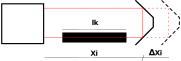
\includegraphics[width=0.8\textwidth]{drawing.pdf}
% \end{figure}

\newpage
\section{Měření}
Změřená frekvence modulačního signálu \(49.98\;kHz\Rightarrow f=49.98\;MHz\) \\
Délka trubic s kapalinami             \(1014\;mm\)
\begin{figure}[H]
	\begin{minipage}[t]{0.35\textwidth}
        \paragraph*{měření~rychlosti~světla~ve~vzduchu}
        \begin{tabular}{|c|c|c|c|c|c|}
            \hline
            č.\;m.                      & 1     & 2     & 3     & 4     & 5     \\ \hline
            \(x_i\;[cm]\)               & 7.1   & 6.8   & 5.5   & 5.0   & 5.0   \\ \hline
            \(x_{i}^{\prime}\;[cm]\)    & 155.6 & 155.4 & 154.5 & 155.0 & 155.1 \\ \hline
            \(\Delta x_{i}\;[cm]\)      & 148.5 & 148.6 & 149.0 & 150.0 & 150.1 \\ \hline
        \end{tabular}
        \\ \\
        \(\Delta x_{v-str}=\sum \frac{x_{i}}{5}=149.24\;cm\)
    \end{minipage}
    \hfill
	\begin{minipage}[t]{0.5\textwidth}
        \paragraph*{měření\;rychlosti\;světla\;v\;kapalině\;1}
        \begin{tabular}{|c|c|c|c|c|c|}
            \hline
            č.\;m.                      & 1     & 2     & 3     & 4     & 5     \\ \hline
            \(x_i\;[cm]\)               & 128.9 & 116.8 & 116.4 & 116.4 & 116.4 \\ \hline
            \(x_{i}^{\prime}\;[cm]\)    & 152.8 & 142.4 & 142.2 & 141.9 & 141.4 \\ \hline
            \(\Delta x_{i}\;[cm]\)      & 23.9  & 25.6  & 25.8  & 25.5  & 25.0  \\ \hline
        \end{tabular}
        \\ \\
        \(\Delta x_{1-str}=\sum \frac{x_{i}}{5}=25.16\;cm\)
    \end{minipage}
\end{figure}
\begin{figure}[H]
	\begin{minipage}[t]{0.35\textwidth}
        \paragraph*{měření\;rychlosti\;světla\;v\;kapalině\;2}
        \begin{tabular}{|c|c|c|c|c|c|}
            \hline
            č.\;m.                      & 1     & 2     & 3     & 4     & 5     \\ \hline
            \(x_i\;[cm]\)               & 108.2 & 108.2 & 111.2 & 111.3 & 108.4 \\ \hline
            \(x_{i}^{\prime}\;[cm]\)    & 140.9 & 141.2 & 140.8 & 141.1 & 140.7 \\ \hline
            \(\Delta x_{i}\;[cm]\)      & 32.7  & 33.0  & 39.6  & 29.8  & 32.3  \\ \hline
        \end{tabular}
        \\ \\
        \(\Delta x_{2-str}=\sum \frac{x_{i}}{5}=33.48\;cm\)
    \end{minipage}
    \hfill
	\begin{minipage}[t]{0.5\textwidth}
        \paragraph*{měření\;rychlosti\;světla\;v\;kapalině\;3}
        \begin{tabular}{|c|c|c|c|c|c|}
            \hline
            č.\;m.                      & 1     & 2     & 3     & 4     & 5     \\ \hline
            \(x_i\;[cm]\)               & 108.1 & 108.0 & 108.1 & 108.1 & 108.3 \\ \hline
            \(x_{i}^{\prime}\;[cm]\)    & 128.4 & 128.9 & 127.8 & 128.7 & 128.8 \\ \hline
            \(\Delta x_{i}\;[cm]\)      & 20.3  & 20.9  & 19.7  & 20.6  & 20.5  \\ \hline
        \end{tabular}
        \\ \\
        \(\Delta x_{3-str}=\sum \frac{x_{i}}{5}=20.4\;cm\)
    \end{minipage}
\end{figure}

Rychlost světla ve vzduchu stanovíme úpravou vzorce (\textbf{3})  z \(\Delta x_{v-str}\) a frekvence \(f\) jako
\\
\begin{displaymath}
    c=f \lambda=f \Delta x_{v-str}\cdot2\cdot2=(49.98\cdot10^{6}\cdot149.24\cdot10^{-2}\cdot4)\;m\cdot s^{-1}=298.4\cdot10^{6}\;m\cdot s^{-1}
\end{displaymath} 
tabulková hodnota je \(299.8\cdot10^{6}\;m\cdot s^{-1}\) a mé měření má tak odchylku \(0.5\;\%\).

\begin{figure}[H]
	\begin{minipage}[t]{\textwidth}
        Rychlost světla v kapalinách stanovíme ze vztahu (\textbf{4})\\
        \begin{displaymath}
            v_{k1}=\frac{c\cdot l_k}{l_k+2\Delta x_{1-str}}=\frac{298.4\cdot10^{6}\cdot 1.014}{1.014+2\cdot25.16\cdot10^{-2}}\;m\cdot s^{-1}=199.4\cdot10^{6}\;m\cdot s^{-1}
        \end{displaymath}
        \begin{displaymath}
            v_{k2}=\frac{c\cdot l_k}{l_k+2\Delta x_{2-str}}=\frac{298.4\cdot10^{6}\cdot 1.014}{1.014+2\cdot33.48\cdot10^{-2}}\;m\cdot s^{-1}=179.7\cdot10^{6}\;m\cdot s^{-1}\\
        \end{displaymath}
        \begin{displaymath}
            v_{k3}=\frac{c\cdot l_k}{l_k+2\Delta x_{2-str}}=\frac{298.4\cdot10^{6}\cdot 1.014}{1.014+2\cdot20.4\cdot10^{-2}}\;m\cdot s^{-1}=212.8\cdot10^{6}\;m\cdot s^{-1}
        \end{displaymath}
        \\
        Index lomu \(n\) u jednotlivých kapalin určíme podle vzorce (\textbf{2}) \\
        \\
\vspace{-7mm}

        \begin{displaymath}
            n_{k1}=\frac{c}{v_{k1}}=\frac{298.4\cdot10^{6}}{199.4\cdot10^{6}}=1.496\;[-]
        \end{displaymath}
        \begin{displaymath}
            n_{k2}=\frac{c}{v_{k2}}=\frac{298.4\cdot10^{6}}{179.7\cdot10^{6}}=1.661\;[-]
        \end{displaymath}
        \begin{displaymath}
            n_{k3}=\frac{c}{v_{k3}}=\frac{298.4\cdot10^{6}}{212.8\cdot10^{6}}=1.402\;[-]
        \end{displaymath}
    \end{minipage}
\end{figure}
\vspace{-11mm}
\section{Závěr}
Na základě meření ve vzduchu jsem stanovil rychlost světla na \(298.4\cdot10^{6}\;m\cdot s^{-1}\) což při porovnání s tabulkovou hodnotou \(299.8\cdot10^{6}\;m\cdot s^{-1}\) znamená odchylku \(0.5\;\%\).
Pomocí takto získané hodnoty jsem stanovil rychlost světla ve třech různých kapalinách na \(199.4\cdot10^{6}\;m\cdot s^{-1}\), \(179.7\cdot10^{6}\;m\cdot s^{-1}\) a \(212.8\cdot10^{6}\;m\cdot s^{-1}\).
Nakonec jsem pomocí stanovených rychlostí určil indexy lomu pro jednotlivé kapaliny jako \(1.496\), \(1.661\) a \(1.402\). 
Podle indexu lomu jsem určil první kapalinu \(n=1.496\) jako roztor cukru (80\%), druhou kapalinu \(n=1.661\) jako těžké flintové sklo a třetí kapalinu \(n=1.402\) jako jako roztor cukru (30\%).
Nepřesnost měření byla pravděpodobně způsobena nepřesným odečtem fázového posunu z Lissajousova obrazce a což způsobilo chybu měření vlnové delky.

\end{document}
